\chapter{System Architecture and Details}
\label{ChapterFive}

\section{Frameworks and Technologies}
\label{FrameworksAndTechnologies}

\section{Database Design and Implementation}
\label{DatabaseDesignandImplementation}

\section{Web Portal}
\label{WebPrtal}

\section{Data Visualization}
\label{DataVisualization}

\section{Decision Support}
\label{DecisionSuport}
%
%\subsection{Quality Metrics Used to Analyze Data Synchronization Platforms}
%\label{QualityMetrics}
%\indent In the process of assessment the quality of data synchronization framework there are some important characteristics that should be measured and interpreted. This evaluation is even more rigorous for systems that are constrained to limited resources, as in the case of mobile devices. In order to perform an analysis of the solution presented in this paper, we have to define quality metrics that are relevant for data synchronization process. 
%\subsubsection{Computation Time}
%\label{ComputationTime}
%\indent Synchronization algorithms require different computational efforts and processing capabilities. This aspect is a key problem for mobile devices that have restricted computational power. In such conditions, the response time of the application can have significant delays reducing the usability and efficiency nonfunctional requirements of the system. This problem is truly essential especially in the case of systems that are using synchronous communication. For asynchronous communication, the problem is reduced as the processing work is done in the background.
%
%\subsubsection{Scalability}
%\label{Scalability}
%\indent Our system is addressed to users of mobile devices. Mobile device has recorded a continuous growth in the last years and it is expected that in the future, users will be more tempted to  number is increasing continuously. This is the reason for which the system should be scalable and able to handle more requests simultaneously. As no access for the server side functionality was not given, we cannot know how the scaling aspect was tackled. 

%\subsubsection{Data Storage}
%\label{DataStorage}
%\indent Even though storage is not a big problem as before for mobile devices, it is not desirable to have an application whose data occupies a big storage space. This metric refers to the actual space occupied by both the database information and the files needed by the application (the images for different brands, products, articles).
%
%\subsubsection{Network Overload}
%\indent Data synchronization involves the transfer of data of different sizes. The problem might be neglectful in the case of small databases, but it becomes important for larger databases. The most undesired option is to update the entire database, but this problem has been previously addressed and we will focus on the network overload in the case of systems that update only entities that are not consistent. \\
%\indent The size of data load affects the time required for the synchronization process and together with the time needed by the synchronization algorithm defines the actual communication time between the mobile device and the centralized server.
%\label{NetworkOverload}
%
%\subsection{Data Storage Evaluation}
%\label{subsec:DataStorageEvaluation}
%\indent A part of the image files, more exactly the ones that correspond to product brands and product groups are fixed and will be saved on the mobile phone together with the application. There is no need to synchronize them.\\
%\indent As the application has to synchronize both data from the database and a part of the files, we will illustrate the space occupied in both cases. These comparison is important also in understanding why we chose to separate data synchronization from file synchronization. Because image files are the same, they can be saved even after the user logs out. In figure 5.1 the space occupied in the case of accounts with only one or several customers associated is presented.\\
%\begin{figure}[ht]
%	\centering
%	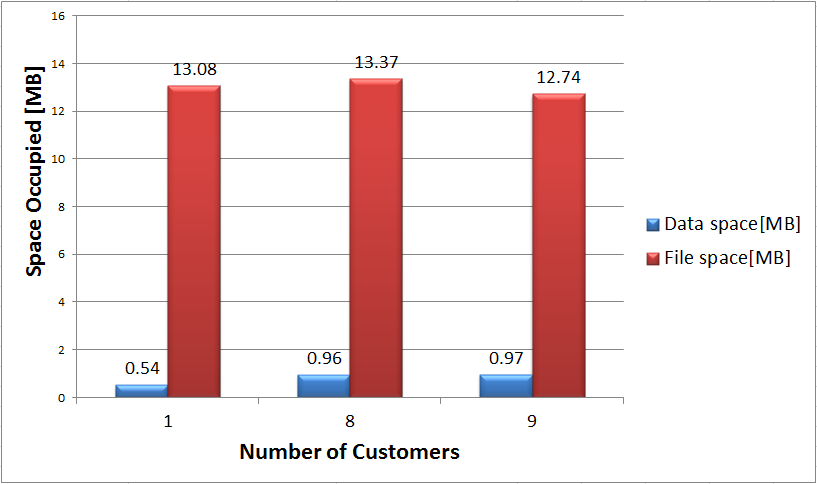
\includegraphics[scale=0.65]{Images/data_storage.png} 
%	\caption[Data Storage for Different Accounts]{Data Storage for Different Accounts}
%	\end{figure}
%\indent As one can see, the space occupied by the data in the database is very small in comparison with the space occupied by the image files. For this reason, it is better to split the synchronization according to data and files. Image files are anyhow rarely changed so there is no need for frequent synchronization.\\
%\indent The size occupied by data varies proportionally with the number of customers associated to the account. This happens because for every customer number, the articles associated to it are stored in a different tables. So in the case of more customers, more article-customer associations are present. \\
%\indent The variation of space occupied by the image files is not relevant as an account with only one customer can have more articles then an account with eight customers but more restrictions. As image files are retrieved for article and products, in the case with accounts with a larger variety of articles, more files are retrieved. This process is independent on the number of customers.
%
%\subsection{Latency Test}
%\label{subsec:LatencyTest}
%\indent The time needed for exchanging the information is directly proportional with the amount of information that has to be exchanged and the Internet connection. It is also dependent on the response time of the server. The tests performed for measuring the necessary time were done on an Internet connection for which the download speed was circa 20 Mbps.\\
%\begin{figure}[ht]
%	\centering
%	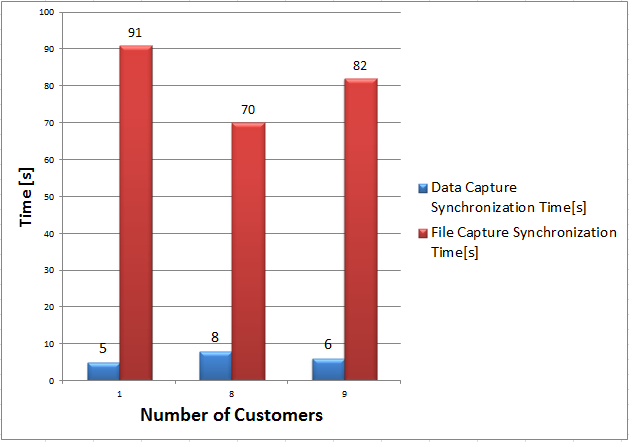
\includegraphics[scale=0.65]{Images/time_performance.png} 
%	\caption[Capture Synchronization Time for Different Accounts]{Capture Synchronization Time for Different Accounts}
%	\end{figure}
%\indent We can clearly observe that data synchronization requires considerably less time synchronization. Capture synchronization retrieves all the data from the server side at log in. Further data synchronization methods require even less time as there is no need to synchronize all the database.\\
%\indent No clear dependency between the synchronization time and the number of customers associated to an account can be depicted. The influence of server's response time affects the total time.\\
%\indent File synchronization takes longer and will be performed rarely in comparison with the data synchronization.\\